\documentclass[a4paper, 12pt]{article}
\usepackage[left=1.5cm, text={18cm, 25cm}, top=2.5cm]{geometry}
\usepackage[utf8]{inputenc}
\usepackage[czech]{babel}
\usepackage{cite}
\usepackage{graphicx}
\usepackage{float}
\usepackage{amsmath}
\usepackage{tikz}
\usepackage{url}
\usepackage{comment}
\newcommand{\myuv}[1]{\quotedblbase #1\textquotedblleft}
\newcommand{\defVal}[1]{$Default=#1$}

\title{Implementace algoritmu Enumeration sort}
\author{Martin Hruška\\xhrusk16@stud.fit.vutbr.cz}

\date{}
\begin{document}

\maketitle

\section{Úvod}
\label{sec:intro}
Enumeration sort je paralelní řadící algoritmus, který může pracovat s~procesory uspořádanými v~mřížce nebo v~lineárním poli.
Tato práce se zabývá implementací varianty algoritmu pro lineární pole procesorů, která řadí
posloupnost obsahující $n$ přirozených čísel z~intervalu $\langle 0,255 \rangle$ dle jejich velikosti za použití $n+1$ procesorů.
Pro implementaci byla použita knihovna \emph{openMPI} a implementačním jazykem bylo C++.
V~tomto dokumentu bude algoritmus napřed
stručně popsán a bude provedena teoretická analýza jeho složitosti (sekce \ref{sec:analysis}),
následně budou popsány v~sekci \ref{sec:impl} implementační detaily,
v~sekci \ref{sec:exprmts} provedené experimenty
a na závěr je uveden sekvenční diagram znázorňující komunikaci jednotlivých procesorů (sekce \ref{sec:seq}).

\section{Popis a analýza algoritmu}
\label{sec:analysis}
V~této sekci bude teoreticky popsán implementovaný algoritmus a následně bude na základě uvedeného popisu provedena
analýza jeho časové složitosti.

Algoritmus Enumeration sort pracuje následujícím způsobem:
\begin{enumerate}
\item Každý vstupní procesor má registry $X, Y, C, Z$ a registr $C$ na úvod nastaví
na hodnotu jedna.
\item Provádí se cyklus o~$2*n$ opakováních, kde v~prvních $k$ cyklech (kde $k\leq n$)
je $k$-tý prvek přiřazen $k$-tému procesoru do registru $X$.
Registry $Y$ postupně prochází vstupní posloupnost tak, že v~každé iteraci cyklu se posune prvek posloupnosti z~daného procesoru
do jeho následníka v~poli procesorů a do prvního procesoru jsou takto nahrávány prvky vstupní posloupnosti.
Procesory v~každém cyklu porovnají hodnoty v~registru $X$ a $Y$ (pokud mají tyto definovány)
a pokud $X < Y$, tak inkrementují registr $C$ o~hodnotu jedna.
V~každém $k$-tém cyklu (kde $k \geq n$) je pak přiřazena hodnota z~registru $X$ ($k-n$)-tého procesoru do registru $Z$ procesoru,
jenž je v~poli procesorů na stejné pozici jako je daná hodnota v~seřazené posloupnosti.
\item V~závěrečném kroku jsou pak v~cyklu hodnoty z~registru $Z$ přesouvány na výstup tak, že je hodnota
z~registru $Z$ jednoho procesoru přenesena do registru $Z$ procesoru, který ho v~poli procesorů následuje.
Z~posledního procesoru v~poli je pak přenesena tato hodnota na výstup.
\end{enumerate}

Nyní přistupme k~analýze časové složitosti algoritmu.
První bod z~popisu algoritmu, tedy inicializace registru $C$ na hodnotu jedna je možno provést v~konstantním čase,
zapsáno v~$O$ notaci jako $O(1)$.
V~druhém bodě je proveden cyklus $2*n$-krát a každou iteraci cyklu lze provést v~konstantním počtu kroků, dohromady tedy
dostáváme složitost $2*n*c=O(n)$, kde $c$ je konstanta udávající počet kroků výpočtu v~těle cyklu.
Třetí bod je cyklus s~$n$ opakováními a každou iteraci cyklu lze provést také v~konstantním počtu kroků, celkem pak $n*c_2=O(n)$,
kde $c_2$ je konstanta udávající počet kroků výpočtu v~těle cyklu.
Celý výpočet má tedy časovou složitost $t(n)=O(1)+O(n)+O(n)=O(n)$.
Počet procesorů nutných k~výpočtu je $n$, a tedy $p(n)=n$.
Cena paralelního řešení $c(n)$ je $p(n)*t(n)=n*O(n)=O(n^2)$.


\section{Implementace}
\label{sec:impl}
Algoritmus byl implementován dle popisu z~předchozí části \ref{sec:analysis} až na změny uvedené v~této části.
V~této sekci budou také popsány některé implementační detaily.

Vstupní posloupnost čísel program načítá ze souboru \emph{numbers}, kde je uložena jako sekvence bytů.
Proto existovaly dvě možnosti implementace samotného algoritmu.
V~první by probíhalo samotné načítání hodnot ze souboru během řadícího cyklu algoritmu prvním (master) procesorem.
Tento přístup by ale byl nevhodný pro další měření rychlosti algoritmu, protože ta by byla
zkreslena režií spojenou s~načítáním dat ze souboru a průběžným zasíláním zpráv s~aktuálním počtem načtených prvků
vstupní posloupnosti ostatním procesorům, které tuto hodnotu potřebují znát kvůli cyklu prováděném v~druhém kroku algoritmu
(viz. popis v~sekci \ref{sec:analysis}).
Toto bylo také potvrzeno implementací této varianty a následnými experimenty.
Proto byla finální implementace provedena druhým způsobem, při němž první procesor (master) načte všechny prvky posloupnosti,
informuje o~jejich počtu ostatní procesory a při samotném řazení posloupnosti jsou pak hodnoty čteny procesorem master přímo z~paměti
a ostatním procesorům rozesílány pomocí zpráv.
Procesor master se poté na vlastním řazení posloupnosti nepodílí.

Samotný algoritmu Enumeration sort byl upraven tak, aby byl schopen řadit posloupnosti i se stejnými čísly.
Toho bylo dosaženo tak, že v~druhém kroku algoritmu (viz. sekce \ref{sec:analysis}) není
pro všechna čísla, která jsou ve vstupní posloupnosti na pozici s~pořadovým
číslem větším, než je pořadové číslo procesoru v~poli procesorů,
provedeno porovnání $X<Y$, ale $X \leq Y$.

\section{Experimenty}
\label{sec:exprmts}

S~vytvořeným programem byly následně provedeny experimenty s~posloupnostmi o~různé délce, tak aby bylo
možné porovnání s~teoreticky odvozenou složitostí výpočtu.
Experimenty byly provedeny na počítači \emph{merlin.fit.vutbr.cz} a čas byl měřen pomocí
metody \emph{MPI::Wtime} (součást knihovny openMPI), která byla volána před samotným začátkem řazení (tedy až po načtení vstupní posloupnosti ze souboru)
a poté po seřazení a uložení výsledku do výstupní posloupnosti.
Obě hodnoty byly od sebe následně odečteny a tím byla získána doba řazení.
Výsledky měření jsou zobrazeny v~grafu na obrázku \ref{fig:exp}.
Červené body v~grafu udávají reálnou dobu v~sekundách, kterou program potřeboval pro seřazení
posloupnosti o~daném počtu prvků.
Zeleně je pak přímka znázorňující funkci $0.0004*n-0.001$, která ilustruje
časovou složitost $O(n)$, jež by měl mít algoritmus teoreticky.
Výsledky jsou průměrem z~deseti měření.

Z~grafu je patrné, že pro posloupnosti, které obsahovaly $6$ až $25$ prvků, odpovídá teoretická časová složitost
experimentálně naměřeným hodnotám.
U~posloupností s~větším počtem prvků než je $25$, mají naměřené hodnoty velký rozptyl, což lze připsat
limitům (jak systémovým, tak výpočetním) testovacího stroje, na němž bylo (v~1. projektu) doporučeno používat kolem $20$ procesorů, a tedy
i testovat posloupnosti o~délce kolem $20$ prvků.
Toto bylo také potvrzeno experimenty prováděnými s~posloupnostmi delšími než $35$ prvků (což je maximum zobrazené v~grafu),
u~nichž rozptyl výsledných časů akorát více rostl.
Je také vidět, že u~malých posloupností, do délky $5$ prvků, byla doba výpočtu výrazně delší.
Byly také provedeny experimenty, při nichž bylo pro tyto kratší posloupnosti použito většího počtu procesorů
a doba výpočtu klesla na očekávané hodnoty.
Přesnou příčinu tohoto jevu se bohužel nepodařilo zjistit, ale lze předpokládat, že se problém může nacházet na
systémové úrovni a souvisí s~prioritou procesu při malém počtu procesorů.
%Z hlediska definice horního odhadu časové složitosti $O$ ale musí platit,
%že funkce časové složitosti roste danou rychlostí (v našem případě lineární) až od určitého hodnoty $n_0$,
%tudíž by v tomto případě platilo $n_0=7$.

Vzhledem k~omezením daným testovacím strojem \emph{merlin} se tedy podařilo ověřit korespondenci mezi odvozenou složitosti
algoritmu a časovou náročností jeho implementace pouze na menším vzorku dat, na němž časová složitost výpočtu rostla lineárně.

\begin{figure}[bt]
\begin{center}
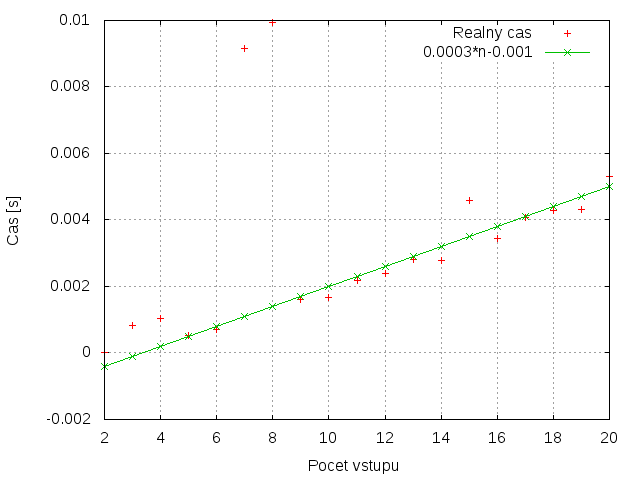
\includegraphics[scale=0.8]{plots/perf.png}
\caption{Doba v~sekundách nutná pro seřazení posloupnosti v~závislosti na její délce.}
\label{fig:exp}
\end{center}
\end{figure}

\section{Sekvenční diagram}
\label{sec:seq}
Na sekvenčním diagramu na obrázku \ref{fig:seq} (obrázek je pro větší čitelnost umístěn na samostatnou stránku)
je znázorněna komunikace mezi procesory.
Proměnné $i,j$ udávají pořadové číslo procesoru v~poli procesorů,
procesor $0$ je procesor na prvním místě v~poli procesorů provádějících řazení (tedy bez procesoru master)
a \emph{všichni} představuje všechny procesory podílející se na řazení.
Pole procesorů použitých pro řazení je v~diagramu indexováno od nuly a procesor master je znázorněn samostatně.
\begin{figure}
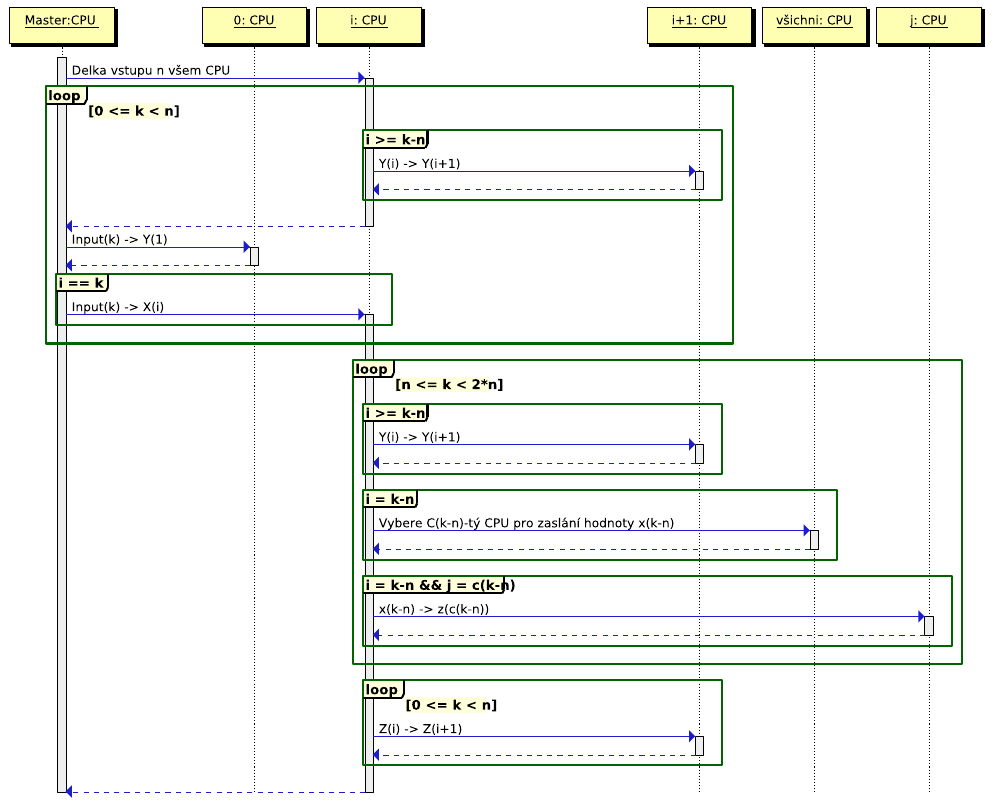
\includegraphics[scale=0.7]{seq.png}
\caption{Sekvenční diagram znázorňující komunikaci mezi procesory}
\label{fig:seq}
\end{figure}

\section{Závěr}
Byl implementován algoritmus Enumeration sort s~lineárním polem procesorů a s~touto implementací byly provedeny
experimenty s~měřením časové náročnosti výpočtu.
Ta byla poté porovnána s~teoreticky odvozenou časovou složitostí a
bylo zjištěno, že rychlost implementace odpovídá teoretické analýze složitosti alespoň na omezeném vzorku dat.
V~práci je také uveden sekvenční diagram popisující komunikační protokol implementovaného algoritmu.

\end{document}
